% mnras_template.tex 
%
% LaTeX template for creating an MNRAS paper
%
% v3.0 released 14 May 2015
% (version numbers match those of mnras.cls)
%
% Copyright (C) Royal Astronomical Society 2015
% Authors:
% Keith T. Smith (Royal Astronomical Society)

% Change log
%
% v3.0 May 2015
%    Renamed to match the new package name
%    Version number matches mnras.cls
%    A few minor tweaks to wording
% v1.0 September 2013
%    Beta testing only - never publicly released
%    First version: a simple (ish) template for creating an MNRAS paper

%%%%%%%%%%%%%%%%%%%%%%%%%%%%%%%%%%%%%%%%%%%%%%%%%%
% Basic setup. Most papers should leave these options alone.
\documentclass[fleqn,usenatbib]{mnras}

% MNRAS is set in Times font. If you don't have this installed (most LaTeX
% installations will be fine) or prefer the old Computer Modern fonts, comment
% out the following line
\usepackage{newtxtext,newtxmath}
% Depending on your LaTeX fonts installation, you might get better results with one of these:
%\usepackage{mathptmx}
%\usepackage{txfonts}

% Use vector fonts, so it zooms properly in on-screen viewing software
% Don't change these lines unless you know what you are doing
\usepackage[T1]{fontenc}

% Allow "Thomas van Noord" and "Simon de Laguarde" and alike to be sorted by "N" and "L" etc. in the bibliography.
% Write the name in the bibliography as "\VAN{Noord}{Van}{van} Noord, Thomas"
\DeclareRobustCommand{\VAN}[3]{#2}
\let\VANthebibliography\thebibliography
\def\thebibliography{\DeclareRobustCommand{\VAN}[3]{##3}\VANthebibliography}


%%%%% AUTHORS - PLACE YOUR OWN PACKAGES HERE %%%%%
\usepackage{indentfirst}
\usepackage{physics}
\usepackage{lineno}
\linenumbers
% Only include extra packages if you really need them. Common packages are:
\usepackage{graphicx}	% Including figure files
\usepackage{amsmath}	% Advanced maths commands
\usepackage{amssymb}	% Extra maths symbols
%%%%%%%%%%%%%%%%%%%%%%%%%%%%%%%%%%%%%%%%%%%%%%%%%%

%%%%% AUTHORS - PLACE YOUR OWN COMMANDS HERE %%%%%

% Please keep new commands to a minimum, and use \newcommand not \def to avoid
% overwriting existing commands. Example:
%\newcommand{\pcm}{\,cm$^{-2}$}	% per cm-squared

%%%%%%%%%%%%%%%%%%%%%%%%%%%%%%%%%%%%%%%%%%%%%%%%%%

%%%%%%%%%%%%%%%%%%% TITLE PAGE %%%%%%%%%%%%%%%%%%%

% Title of the paper, and the short title which is used in the headers.
% Keep the title short and informative.
\title[Metacalibration with Roman High-Latitude Imaging Survey]{Weak gravitational lensing shear estimates with \textsc{metacalibration} for the High-Latitude Imaging Survey Program of the \emph{Roman} Space Telescope}

% The list of authors, and the short list which is used in the headers.
% If you need two or more lines of authors, add an extra line using \newauthor
\author[M. Yamamoto et al.]{
Masaya Yamamoto,$^{1}$\thanks{E-mail: masaya.yamamoto@duke.edu}
Michael A. Troxel,$^{1}$
Mike Jarvis,$^{2}$
Rachel Mandelbaum,$^{3}$
Christopher Hirata$^{4,5,6}$
\\
% List of institutions
$^{1}$Department of Physics, Duke University, Durham, NC, 27710\\
$^{2}$Department of Physics and Astronomy, University of Pennsylvania, Philadelphia, PA 19104, USA\\
$^{3}$McWilliams Center for Cosmology, Department of Physics, Carnegie Mellon University, Pittsburgh, Pennsylvania 15213, USA\\
$^{4}$Center for Cosmology and Astro-Particle Physics, The Ohio State University, 191 West Woodruff Avenue, Columbus, OH 43210, USA\\
$^{5}$Department of Physics, The Ohio State University, 191 West Woodruff Avenue, Columbus, OH 43210, USA\\
$^{6}$Department of Astronomy, The Ohio State University, 140 West 18th Avenue, Columbus, OH 43210, USA\\
}

% These dates will be filled out by the publisher
\date{Accepted XXX. Received YYY; in original form ZZZ}

% Enter the current year, for the copyright statements etc.
\pubyear{2015}

% Don't change these lines
\begin{document}
\label{firstpage}
\pagerange{\pageref{firstpage}--\pageref{lastpage}}
\maketitle

% Abstract of the paper
\begin{abstract}
We investigate the performance of the \textsc{metacalibration} scheme in the framework of the \emph{Nancy Grace Roman} Space Telescope (\emph{Roman}) image simulations. By comparing non-calibrated results from the previous work, shear calibration bias can be reduced significantly with \textsc{metacalibration}. Exploring shear bias is a robust way to test the requirements of the instrument and the overall weak lensing survey strategy. The weak lensing program of \emph{Roman} mission requires the galaxy shapes to be calibrated within about 0.03\%. To reach this goal, we can test our calibration scheme with these simulations and can isolate the sources where these residual shear biases come from, (whether it is the algorithm or detector physics). We incorporate several new updates that are more realistic and necessary to calibrate shear with a better precision relative to the previous version of the simulations. Without the coadditions of the single epoch images, across all three filters we are able to achieve the multiplicative bias of 0.70 per cent within 1.8 $\sigma$ with the current simulation volume. Meanwhile, average additive bias is not consistent with zero due to the strong correlation with the input PSF for one of the spin-2 component directions but consistent with zero for the other direction. This is worse for coadded images. We find no evidence that shape calibration becomes worse with decreasing image sampling factor based on the Nyquist sampling theorem. Overall, within the current simulation volume, we find that \textsc{metacalibration} can calibrate shapes with zero systematics on relatively undersampled images that \emph{Roman} will produce. In the future, we will need to substantially increase the simulation volume by 8 to reach the accuracy necessary for the program. 
\end{abstract}

% Select between one and six entries from the list of approved keywords.
% Don't make up new ones.
\begin{keywords}
gravitational lensing: weak -- cosmology: observations -- techniques: image processing
\end{keywords}

%%%%%%%%%%%%%%%%%%%%%%%%%%%%%%%%%%%%%%%%%%%%%%%%%%

%%%%%%%%%%%%%%%%% BODY OF PAPER %%%%%%%%%%%%%%%%%%

\section{Introduction}

Since the formulation of the physical cosmological model, more observational evidence has shown that the contents of the universe are mostly in the dark sector (\citealt{2020A&A...633A..69H, 2018PhRvD..98d3528T, 2019PhRvL.122q1301A, 2019PASJ...71...43H, 2021A&A...645A.104A}). Within the dark sector, dark energy accounts for the accelerating expansion of the universe (e.g., \citealt{1998AJ....116.1009R, 1999AIPC..478..129P}) and the combination of dark energy and dark matter which only interacts with the same kind are responsible for the growth of the large-scale structure (\citealt{2015RPPh...78h6901K, 2017grle.book.....D}). The growth can be studied by carefully reconstructing the paths of the light leaving distant galaxies and going through the region where masses concentrate in the universe; this physical phenomenon is called gravitational lensing. “Weak” gravitational lensing causes a slight distortion to intrinsic galaxy shapes, and measuring the distorted shapes describes the gravitational shear field the light passes through. By using millions of these gravitationally lensed galaxies we can explore the matter density and the amplitude of matter fluctuation in the universe (e.g., \citealt{2001PhR...340..291B}). Measuring these quantities eventually help us learn the history of the development of the structure. For that reason, weak lensing is and will continue to be one of the key probes in the current and next-decade imaging surveys to constrain cosmological parameters with high precision. \par


Due to the subtlety in the lensing effect and its systematics dominant nature in the “weak” regime, observational efforts have been challenging. Over the past decade, large international collaborations such as the Dark Energy Survey\footnote{\url{http://www.darkenergysurvey.org/}} (DES: \citealt{2005astro.ph.10346T}), the Hyper Supreme-Cam\footnote{\url{http://hsc.mtk.nao.ac.jp/ssp/}} (HSC: \citealt{2018PASJ...70S...4A}), and the Kilo-Degree Survey\footnote{\url{http://kids.strw.leidenuniv.nl/}} (KiDS) have been successful at constraining the cosmological parameters, and the precision in calibrating the shapes of distant galaxies has reached a few percent (\citealt{2020arXiv201103408G, 2020arXiv201208567M, 2021A&A...645A.105G}) (include most recent HSC catalog). As we cover more areas in the sky and develop better tools (observatories and algorithms), we find more galaxies and we have already reached to the point where statistical and systematic uncertainties are comparable. Thus, the next-decade legacy surveys, the Stage IV surveys (\citealt{2006astro.ph..9591A}) such as Euclid\footnote{\url{ http://sci.esa.int/euclid}} (Euclid Study Scientist & the Science Advisory Team 2010), the Vera C. Rubin Observatory Legacy Survey of Space and Time\footnote{\url{ http://www.lsst.org}} (LSST: \citealt{2009arXiv0912.0201L, 2019ApJ...873..111I}), and \emph{Nancy Grace Roman} Space Telescope\footnote{\url{https://roman.gsfc.nasa.gov}} (\emph{Roman}: \citealt{2015arXiv150303757S}) require even better control of systematics. In order to manage the systematic uncertainties, we must develop realistic image simulations, apply the shape measurement on the simulated images, and determine any potential systematic effects and the strategy of mitigating them.  


Based on our current knowledge, systematic biases for weak lensing science, both observational and astrophysical, could occur throughout imaging surveys (\citealt{2018ARA&A..56..393M}). Particularly, observational systematics can be found in, 
\begin{itemize}
    \item observing strategy
    \item instrumentation effects such as Brighter-Fatter Effect
    \item post-processing pipeline such as image coaddition and object detection
    \item cosmological inference 
\end{itemize} 


In this study, we focus on shear calibration bias, which describes the relationship between gravitational lensing shear and measured galaxy shapes. In the limit of weak lensing ($\lvert\gamma\rvert\ll1$), the ensemble average of ellipticities $\langle e \rangle$ of galaxy shapes is directly related to the shear field $\gamma$, and the estimated shear can be written as a linear model with multiplicative ($m_{i}$) and additive bias ($c_{i}$) as described in the equation below. (\citealt{2006MNRAS.368.1323H, 2006MNRAS.366..101H, 2007MNRAS.376...13M}) 
\begin{equation}
    \gamma^{obs}_{i} = (1+m_{i})\gamma^{true}_{i} + c_{i}, 
    \label{eqn:linear}
\end{equation}
where i=(1,2) and $\gamma^{obs}_{i}$ is the two-component observed shear after calibrations and $\gamma^{true}_{i}$ is the true shear. This shear bias arises for various reasons. For space-based surveys, it can be mainly introduced in places such as PSF modelling, blending, and the undersampling of the image (e.g., \citealt{2018ARA&A..56..393M}). Additionally, complex detector effects such as brighter-fatter effect are the potential sources of bias (\citealt{2013MNRAS.429..661M}), where it is shown that for \emph{Roman} the effect of persistence will not be an issue (\citealt{2021arXiv210610273L}). Qualitatively, if the recovered shear is biased by 1$\%$ (m=1$\%$), $S_{8} = \sigma_{8} \sqrt{\Omega_{m}/0.3}$ would be biased about 1.5$\%$ in the final cosmology result. Thus, quantifying this shear bias before the survey is extremely important. \par


Several shear calibration and bias mitigation efforts have been proposed by STEP (\citealt{2006MNRAS.368.1323H, 2007MNRAS.376...13M}) and GREAT (\citealt{2010MNRAS.405.2044B, 2013ApJS..205...12K, 2015MNRAS.450.2963M}) challenges, to meet the requirements for the current imaging surveys. In particular, one of the state-of-the-art self-calibration methods, \textsc{metacalibration} (\citealt{2017arXiv170202600H, 2017ApJ...841...24S}) has been shown to be able to reduce the significant of shear bias. It has also confirmed that the shear can be calibrated with \textsc{metacalibration} at a-few-percent level in DES (\citealt{2018MNRAS.481.1149Z, 2020arXiv201103408G}), without accounting for galaxy blending. Tackling the issue of blending is on the way of Y6 DES analysis with the shear-dependent detection and calibration technique (\textsc{metadetect}; \citealt{2020ApJ...902..138S}). While the major advantage of \textsc{metacalibration} is that it can be directly applied upon real galaxy images, which does not depend on galaxy morphology in simulations, the limitations for future surveys are not well-known. One possible limitation might lie in the effect of the undersampled images, because future space-based surveys like \emph{Euclid} and \emph{Roman} have such a small pixel scale that galaxy images will not be Nyquist sampled at native resolution (\citealt{2013PASP..125.1496S}) based on the Nyquist-Shannon Sampling Theorem. We define the sampling factor of each filter in \emph{Roman} to be, 
\begin{equation}
    Q = \frac{\lambda_{min}N_{f}}{p}, 
    \label{eqn:sampling}
\end{equation}
where $\lambda_{min}$ is the shortest wavelength of the incident light of the filter, $N_{f}$ is the focal ratio of the telescope ($N_{f}=7.8$ for \emph{Roman}) and $p$ is the pixel spacing of the sensor ($p=10\mu m$ for \emph{Roman}). The image with the sampling factor, $Q < 2$, is not Nyquist sampled and reffered to as the undersampled image. It is problematic to measure galaxy shapes solely from the undersampled images, because the \emph{Roman} PSF that will be used to recover the shapes is also undersampled and has a complex structure, not simply Gaussian. It is, therefore, necessary to build a robust strategy that can reconstruct better sampled PSF to allow unbiased shape measurement. 


Recently, Kannawadi et al. (2021) addressed this potential issue of the limitations of \textsc{metacalibration} on undersampled images on \emph{Euclid} image simulations and found that for \emph{Euclid} mission the shear estimate is biased about 1$\%$ (\citealt{2021MNRAS.502.4048K}). They mentioned that his result could be extended to the \emph{Roman} mission due to their similarities in the instruments and for \emph{Roman} they predicted the multiplicative bias was more than 1\% for H158 and F184 filters. Regardless of this extended result, we should validate if \textsc{metacalibration} is non-biased with the image simulations specifically made for the \emph{Roman} mission. Our work is based on the image simulation suite of the \emph{Roman} Space Telescope developed by \citet{2021MNRAS.501.2044T}, where we render star and galaxy images from \texttt{GalSim}\footnote{\url{ https://github.com/GalSim-developers/GalSim}} (\citealt{2015A&C....10..121R}). With a few simulation updates and an implementation of \textsc{metacalibration}, we can start to explore if the shear calibration goal of the High-Latitude Survey program for Roman ($m=~3.2\times10^{-4}$) (\citealt{2019BAAS...51c.341D}) can be achieved. \par


This paper is organized as follows. We briefly discuss the simulation suite details we used and the updates we implemented for this project in Sec.~\ref{sec:sims}. Then, in Sec.~\ref{sec:methods}, we show how coadditions of single exposure postage stamps are produced and how shape measurements are completed using \textsc{metacalibration}. We present the galaxy catalog properties and calibration results for single-band and multiband measurements in Sec.~\ref{sec:results}. Finally, in Sec.~\ref{sec:discussion}, we discuss how we will be able to constrain the shear bias better in terms of further updates in the image simulations and what we can conclude from this study. 


\section{Simulations}
\label{sec:sims}
In this section, we briefly summarize the full simulation details from building a truth catalog to measuring galaxy shapes. Then we describe the simulation updates that are implemented particularly for this work.
\subsection{Simulation Summary}
\label{subsec:imsim}
The base of our image simulations of the \emph{Roman} Space Telescope is the \emph{Roman} simulation suite\footnote{\url{ https://github.com/matroxel/roman_imsim}} developed by \citet{2021MNRAS.501.2044T}, which renders realistic galaxy and star images on 18 Sensor-Chip Assemblies (SCAs) of a 2.5$\times$2.5 deg$^{2}$ patch of the sky provided the observing strategy for the 5-year reference mission and Cycle7 specifications\footnote{\url{https://roman.gsfc.nasa.gov/science/Roman_Reference_Information.html}}. We begin by creating a truth catalog using the simulated galaxy distribution from the Buzzard simulation (\citealt{2019arXiv190102401D}), photometric galaxy catalog sampled from the CANDELS survey (e.g., \citealt{2019ApJ...877..117H}), and Milky Way simulation (Galaxia; \citealt{2011ApJ...730....3S}) for star positions and magnitudes. Then, the following properties are applied to each galaxy.
\begin{itemize}
    \item positions (RA, Dec)
    \item photometries for each \emph{Roman} filter (F184/H158/J129/Y106)
    \item intrinsic galaxy shapes and random orientations
    \item flux ratios of de Vaucouleurs bulge, exponential disk, and star-forming knots
    \item artificial gravitational lensing shears
\end{itemize} 
Within the identical realizations of the simulation, we produce four truth catalogs using four sets of gravitational shears ($e_{1}$, $e_{2}$)=\{(+0.02, 0.00), (-0.02, 0.00), (0.00, +0.02), (0.00, -0.02)\}. This approach helps us to reduce shape and measurement noise when taking the difference in recovered shapes to compute multiplicative bias (\citealt{2019A&A...621A...2P}). 


The next step of the process is to create postage stamps and SCA images using \texttt{GalSim}. In this stage, Point-Spread Function (PSF) is convolved with the stamps. Here, the \emph{Roman} PSF is rendered using the \texttt{galsim.roman} module under \texttt{GalSim}, which has implemented \emph{Roman}-specific instrument properties such as the PSF and World Coordinate System (WCS). The module is able to estimate an object position on the sky in RA, Dec using the \emph{Roman} WCS and produce the \emph{Roman} PSF which, for example, correctly describes the diffraction spikes pattern made by the struts and camera in the pupil plane. 



After we generate the object stamps across all the SCAs and pointings, we create Multi-Epoch Data Structure (MEDS) files in which each unique object dictionary contains information of all the exposures. These MEDS files are generated according to the Hierarchical Equal Area isoLatitude Pixelisation (HEALPix) of $n_{side}=512$. These MEDS files contain all objects that are located in the area of the sky partitioned according to a HEALPix of $n_{side}$=512. Once the objects are sorted in MEDS files, we pass them and the corresponding PSF for the SCA to a shape measurement. We pass these multiple exposures with corresponding PSFs to \textsc{ngmix}\footnote{\url{ https://github.com/esheldon/ngmix}} to fit the galaxy shapes with the Gaussian mixture fitting method (\citealt{2014MNRAS.444L..25S}). This shape measurement process produces shape catalogs from which the shear calibration bias can be calculated with \textsc{metacalibration}.

\begin{figure}
	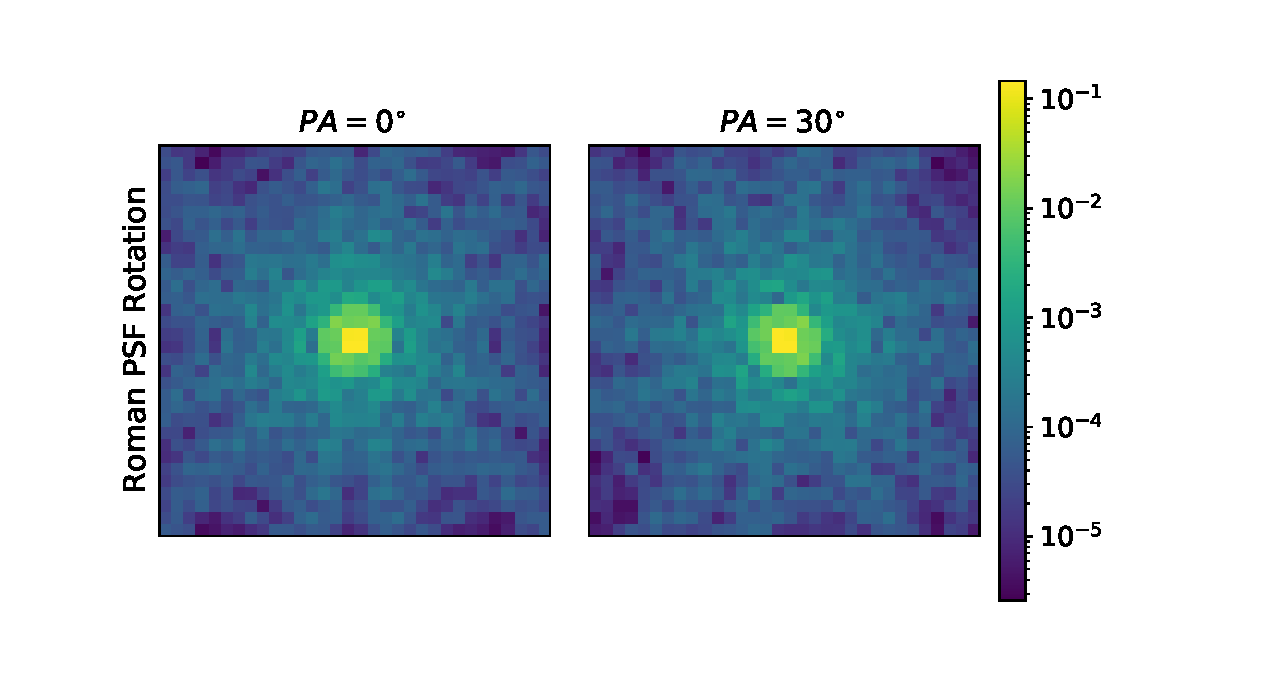
\includegraphics[width=\columnwidth]{figure1.pdf}
	\vspace*{-3mm}
    \caption{The rotation of the Roman PSF produced from the \texttt{galsim.roman} module. Position angle (PA) which determines the rotation of the telescope is $0^{\circ}$ and $30^{\circ}$. The rotation of the PSF is particularly important when an object has multiple exposures and needs to be coadded. If each galaxy image is rotated but each PSF is not, the coadded PSF would have a particular pattern and its shape would not be averaged down. By correctly rotating the PSF that is convolved with galaxy images, the effect of the PSF on the recoverd galaxy shape will be less.}
    \label{fig:psfrot}
\end{figure}

\begin{figure*}
	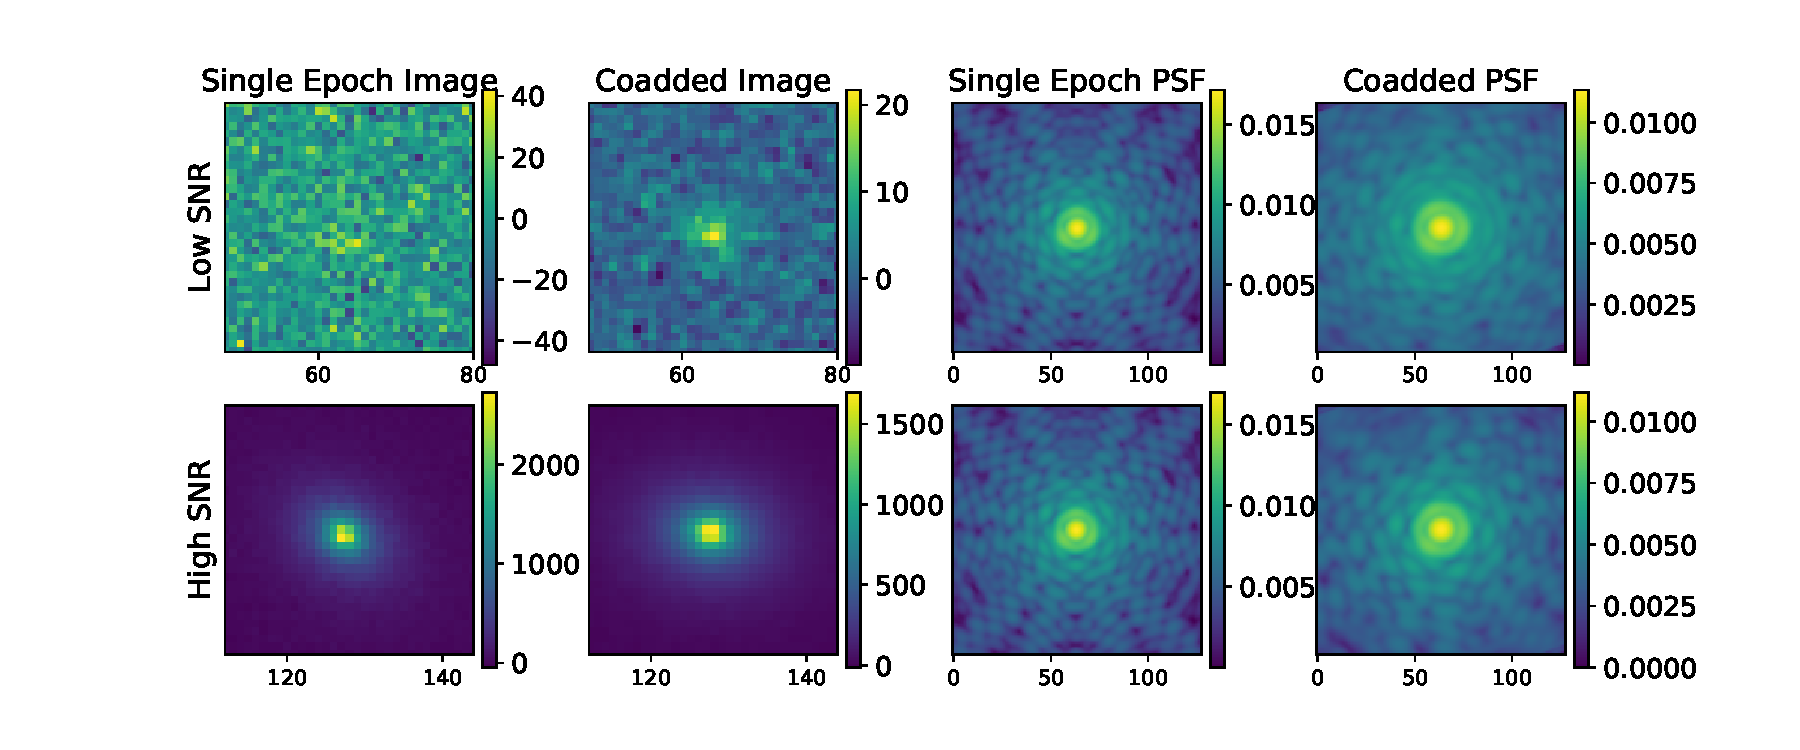
\includegraphics[width=\textwidth]{figure2.pdf}
	\vspace*{-10mm}
    \caption{The top row shows the first entry of the single epoch images and its coadded image, single and coadded oversampled PSF for an object with low signal-to-noise ratio (S/N=9.69). The bottom row shows the same for an object with high signal-to-noise ratio (S/N=1552.97).}
    \label{fig:singlecoadd}
\end{figure*}


\subsection{Simulation Updates}
In order to accomplish science goals, and build and test the pipelines of weak lensing program in \emph{Roman}, we must keep updating the simulations to be more realistic. Along the way to test calibrating shears using \textsc{metacalibration}, we have implemented and made updates to the following parts of the simulation framework. 
\begin{itemize}
    \setlength\itemsep{1em}
    \item \textbf{Saturation Cuts}:
    We have implemented the pixel saturation of 100,000 electrons. This value is an approximate pixel saturation but in the next generation of the simulations we will use the true saturation from the flight candidate detectors. 
    \item \textbf{Rotation of the \emph{Roman} PSF on the sky}:
    In the study by Troxel et al. (2021), the rotations of the \emph{Roman} PSF with respect to the telescope rotation were not engaged properly by \texttt{galsim.roman} module. Since a non-rotating PSF could trigger a preferred direction in the shapes when being deconvolved, we believe that this contributed to the non-zero multiplicative bias. There has been an update in \texttt{galsim.roman} module to correctly rotate the PSF given the WCS on the SCA. Figure \ref{fig:psfrot} shows a toy PSF of the same pointing but with a different rotation angle of the telescope. 
    \item \textbf{Single-band and multiband Coadds}: 
    We have added and modified the postage stamp coadds (\texttt{psc}) algorithm\footnote{\url{https://github.com/esheldon/psc}} to create coadditions of single-epoch postage stamps. Coadds are usually performed to enhance the signal-to-noise ratio (S/N) of an object and mitigate the potential systematics for an accurate shape measurement. If we take advantage of fitting an object in the coadd instead of fitting multiple images of each object in each filter, we can save a factor of 6 in computing time, which is the average number of exposures from the reference survey. Additionally, coadding is one way to reduce the effect of the undersampling of the images since by coadding multiple exposures the product is naturally better sampled. Thus, for these reasons, we must utilize a coadding scheme for the \emph{Roman} galaxies. We can turn this on and off so that the effect of undersampling is clear. The detailed overview of the coadd process in \texttt{psc} is in Sec. \ref{subsec:psc}. 
    \item \textbf{\textsc{metacalibration} implementation}: We used \textsc{metacalibration}\footnote{\url{https://github.com/esheldon/ngmix/wiki/Metacalibration}} bootstrapper method, which is a wrapper class to run measurements in the \textsc{ngmix} package and is used extensively to produce weak lensing shape catalog in DES Y3 analysis. \textsc{metacalibration} process takes place after making coadded images, if applicable for the coadd measurements. With this calibration method, we hope to significantly reduce some of the shear calibration bias Troxel et al. (2021) measured. The detailed overview of \textsc{metacalibration} can be found in Sec.\ref{subsec:mcal}. 
    %\item (Any other changes?)
\end{itemize}


%\subsection{Simple Simulations}
%\label{subsec:simplesim}
%The purpose of the simple simulations is to verify that there are no systematic biases at the basic levels of the simulation (e.g., no complex detector effects). The simple simulation is based on the real observational pointing strategy, and we use the real Sensor-Array Chips (SCAs) scheme, the band filters and the pixel scale as basic Roman specifications.

\section{Post-catalog Processes}
\label{sec:methods}
Our goal is to show that the recovered shapes with \textsc{metacalibration} are non-biased. In order to do so, we need to build a measurement pipeline within the simulation framework that contributes to the final measurement. In this section, we present in detail how coadds are produced with \texttt{psc} from the undersampled single-epoch images, how \textsc{metacalibration} calibrates shapes, and how we measure the shear calibration bias from the \textsc{metacalibration} catalog. 


\subsection{Postage Stamp Coadds}
\label{subsec:psc}
Coaddition is the process that reconstructs a Nyquist-sampled image out of multiple exposures of an object. While this process can benefit in increasing the S/N value of an object and reducing the impact of pixel noise, several challenges need to be addressed for images that are taken with equatorial mount telescopes, which can only move vertically and horizontally, and for images with telescopes that can rotate. When the rotation is introduced, this coadding process becomes more complex to interpolate the image to stack pixel grid. While coaddition could introduce systematic bias due to the complexity of the original PSF and its interpolation scheme, the undersampling of the images can be overcome. We describe our coaddition pipeline that is based on \texttt{psc}.


We reconstruct the Nyquist-sampled image from multiple exposures in MEDS files. For the coaddition of the PSF, we choose to coadd the image with the oversampled PSF over the undersampled original PSF. We oversample the original PSF by a factor of 4 to simulate the better sampled PSF that \emph{Roman} will eventually produce when it constructs the PSF from the full focal plane. It will be highly resolved than native pixel scale. For each exposure of the object we render the \emph{Roman} PSF with a stamp size of 32 pixels at the galaxy centroid. We modified the original code to improve performance of our algorithm, and these modifications are listed below with the general coadding process in \texttt{psc}. 

The algorithm: 
\begin{enumerate}
    \setlength\itemsep{1em}
    \item Finds the wcs of the first exposure of the object.
    \item Translates the original wcs to a flat wcs, because it produces stable results with \textsc{ngmix}.
    \item Creates the coadd stamp with 0.8 $\times$ original pixel scale. We scale the original pixel scale of the final coadd stamp to minimize the effect of undersampling. We noticed that too much oversampling can introduce the artifacts into the structure of the PSF. 
    \item Creates the interpolated image with \texttt{GalSim} with the center offset for each image with \texttt{lanczos3} resampling method. Out of several interpolation methods we tried, \texttt{lanczos3} produced the best coadd of the PSF.
    \item Recreates the coadded noise image from the weight of the original weight map.
\end{enumerate}


Figure \ref{fig:singlecoadd} shows an example of the simulated single-epoch and coadded images and PSFs for objects with low and high S/N. Note that the shape and struts pattern in the original PSF can be washed out by coadding the rotationally dithered PSFs. 


Before we calibrate and measure shapes with \textsc{ngmix}, we downsample the high-resolution PSF to the original pixel size. Figure \ref{fig:coadd_oversample_res} shows the coadded oversampled PSF and the then-downsampled PSF, and their differences. We downsampled the oversampled PSF (128 x 128 pixels) by summing 4 square-pixels and creating the original size PSF (32 x 32 pixels), in order to ensure that the shape fit with \textsc{ngmix} can be processed. Since a better sampled PSF generally enables the shape of the PSF to be more isotropic, from the difference image in Figure \ref{fig:coadd_oversample_res}, we can state that the original PSF has an anisotropic shape, which can lead to biased shape measurement. 

\begin{figure}
	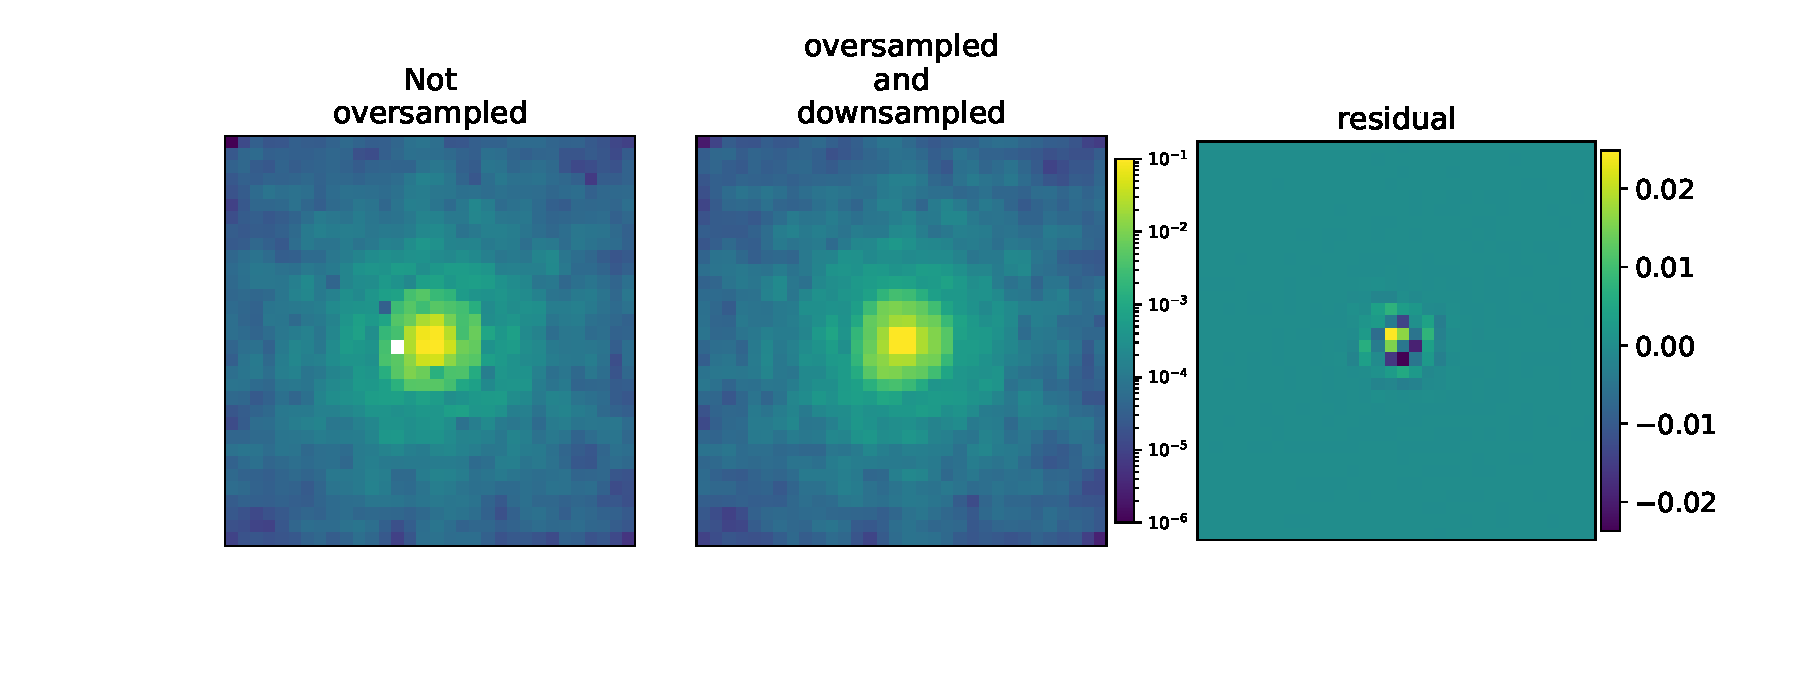
\includegraphics[width=\columnwidth]{figure3.pdf}
    \vspace*{-5mm}
    \caption{The left and middle panel of the figure illustrates the coadded \emph{Roman} PSF at its native pixel scale and the coadded PSF with a pixel scale that is smaller by a factor of 4. These are visualized in a log scale. The right panel shows the difference image between the two PSFs. }
    \label{fig:coadd_oversample_res}
\end{figure}

Finally, Figure \ref{fig:single_to_coadd_rgb} shows the coadd products in different bandpasses for a relatively high S/N object. It is worth noting that the multiband PSF is the oversampled version for a visualization purpose. 

\begin{figure*}
	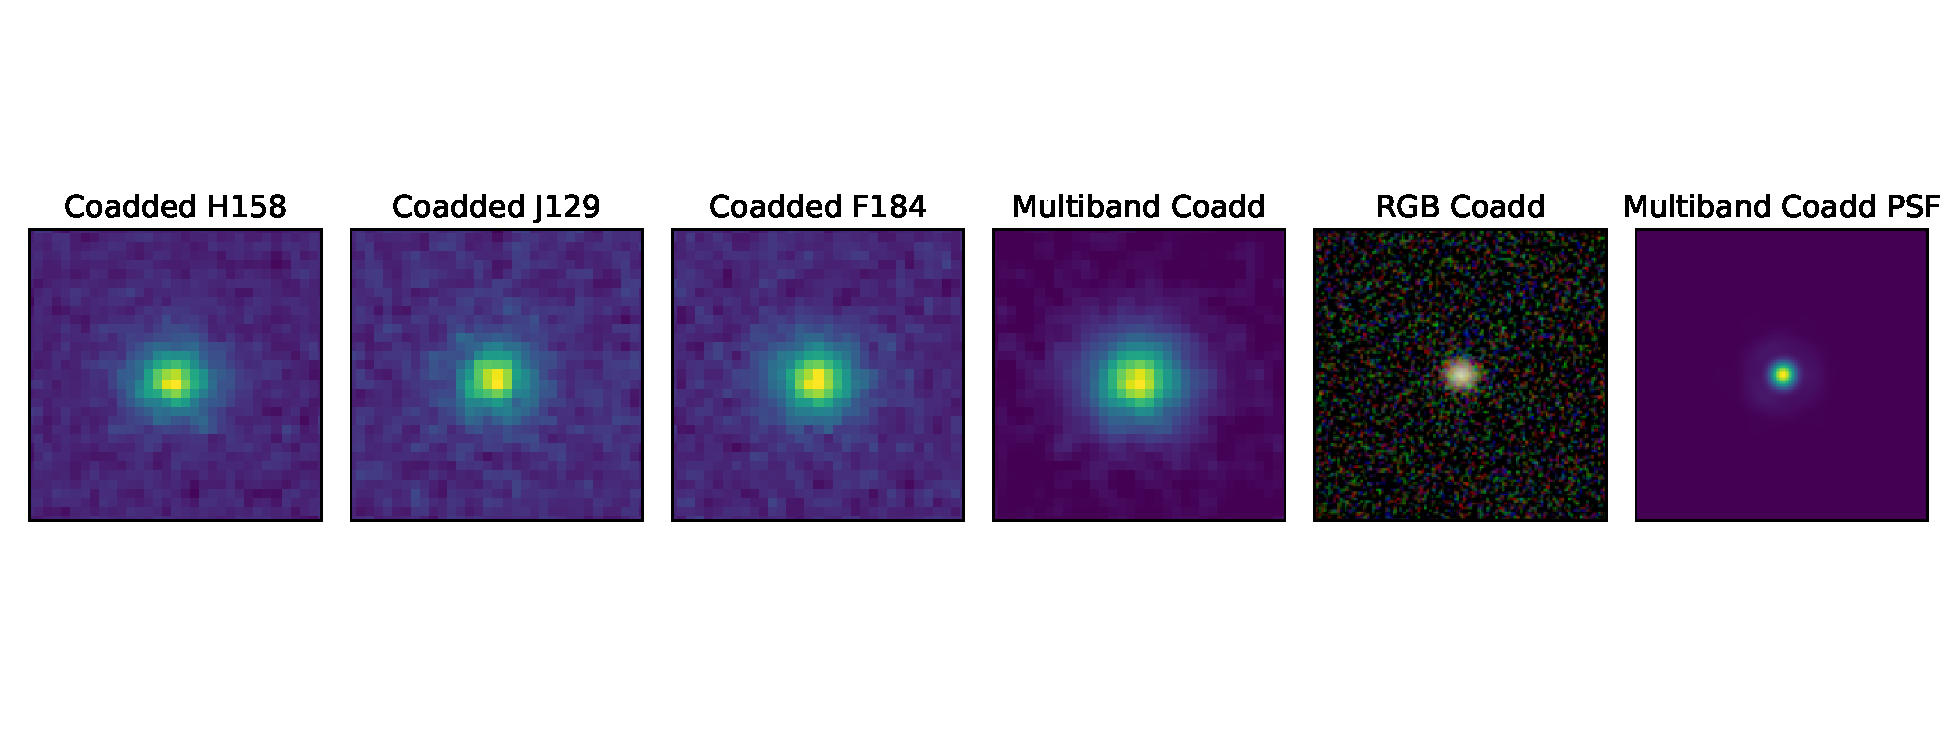
\includegraphics[width=\textwidth]{figure4_og.pdf}
    \vspace*{-20mm}
    \caption{The left 3 panels show an example of the coadded galaxy images for each filter. The S/N for each filter is S/N=2292, 1558, 1336. The 4th and 5th panels show the multiband coadd images of the same object; each with xxx scale and RGB scale. The S/N of the image is S/N=1755. Finally, the right-most panel shows the coadded oversampled PSF with the original scale.}
    \label{fig:single_to_coadd_rgb}
\end{figure*}

\par

\subsection{Shape measurement with \textsc{metacalibration}}
\label{subsec:mcal}
Once we construct the coadds from the galaxy catalogs to recover the shear signal, we feed them into the \textsc{metacalibration} process. The bootstrapper method in \textsc{ngmix} wraps the \textsc{metacalibration} and the shape fit steps. The priors passed to the fit are listed below. 

\begin{table}
    \centering
    \begin{tabular}{|p{3cm}||p{3cm}|p{3cm}|p{3cm}|}
    \hline
    Prior & Value \\
    \hline
    Pixel centroid offset & 0 < $p_{x,y}$ < 0.11\\
    Shear & $|g|=1.0$, $\sigma_{|g|} = 0.3$\\
    Half-light radius & $10^{-5}$ < T < $10^{4}$\\
    Flux fraction of the bulge component & $\langle f\rangle = 0.5$, $\sigma_{f} = 0.1$\\
    Total flux & $0$ < F < $10^{6}$\\
    \hline
    \end{tabular}
    \caption{List of prior values used for the Gaussian mixture fit.}
    \label{tab:priors}
\end{table}


Once we have the \textsc{metacalibration} catalog, we can calculate shear calibration bias from the measured object ellipticities, \vb*{e} = ($e_{1}$, $e_{2}$). The observed ellipticities can be approximated using a Taylor expansion around the two-component shear, $\vb*{\gamma}=0$. Higher terms here can be dropped assuming the gravitational shear is small. It is also known that \textsc{metacalibration} works under the same assumption, otherwise the recovered shear would be biased. It is challenging to find a good input shear that results in higher S/N of an object and unbiased shape measurement. We verify that our input gravitational shear is unbiased in \textsc{metacalibration} framework and the uncertainty in the recovered shape is small enough by constructing the same but simpler framework of the fiducial image simulations which renders Gaussian profile galaxy and PSF on the \emph{Roman} pixel scale cutout image without any detector effects. Figure \ref{fig:metacal_shear_linear} demonstrates that even with the simple enough simulations \textsc{metacalibration} becomes biased after $g=0.05$ since the assumption is starting to break down. 
\begin{equation}
    \vb*{e} = \vb*{e}\rvert_{\vb*{\gamma}=0} + \frac{\partial \vb*{e}}{\partial \vb*{\gamma}}\bigg\rvert_{\vb*{\gamma}=0}\vb*{\gamma} + \ldots
\end{equation}
From this expression, the shear response matrix can be defined as, 
\begin{equation}
    \vb*{R} \equiv \frac{\partial \vb*{e}}{\partial \vb*{\gamma}}\bigg\rvert_{\vb*{\gamma}=0} = 
    \begin{pmatrix}
        \partial e_{1}/\partial \gamma_{1} & \partial e_{2}/\partial \gamma_{1} \\ 
        \partial e_{1}/\partial \gamma_{2} & \partial e_{2}/\partial \gamma_{2}
    \end{pmatrix}. 
\end{equation}
For each redshift bin, the ensemble mean of measured ellipticities $\langle\vb*{e}\rangle$ is computed. Since we expect galaxies in the redshift bin to be randomly oriented such that $\langle\vb*{e}\rangle\rvert_{\vb*{\gamma}=0}=0$, we have a relationship between the measured ellipticities and the input shear in the simulations, 
\begin{equation}
    \langle\vb*{e}\rangle \approx \langle \vb*{R}\vb*{\gamma} \rangle. 
\end{equation} 
In actual observations, the observable is the galaxy shapes $\langle\vb*{e}\rangle$ and we can take advantage of image simulations and calculate the shear response of the particular calibration technique we employ, and finally compute the gravitational lensing shear signal $\langle\vb*{\gamma}\rangle$. 


\textsc{metacalibration} creates one unsheared and four artificially-sheared images of each galaxy stamp. Each is deconvolved with the original PSF, unsheard or sheared with the gravitational shear of $\gamma=0.01$ in four directions ($+g1$, $-g1$, $+g2$, $-g2$) and re-convolved with a new slightly larger isotropic, Gaussian PSF. In our simulation framework, we know the exact input shear and five measured galaxy shapes for each galaxy produced by \textsc{metacalibration} and fitted with the Gaussian mixture method in \textsc{ngmix}. We can calculate the ensemble mean of the shear response from the five versions of \textsc{metacalibration} catalog with the equation below. 


\begin{equation}
    \langle\vb*{R_{ij}}\rangle = 
    \frac{\langle e^{+}_{i} - e^{-}_{i} \rangle}{\Delta\gamma_{j}}, 
\end{equation}
where $e^{+}_{i}$ and $e^{-}_{i}$ is the $i$-th component of the galaxy ellipticity where positive ($+$) or negative ($-$) shear is applied in $i$-th direction. 


Then, this shear response is used to compute the multiplicative ($\vb*{M}$) and additive ($\vb*{C}$) bias using the linear shear bias model (\ref{eqn:linear}). 


\begin{equation}
    \small
    \vb*{M_{ij}} = 
    \frac{\langle e^{+}_{i}/R_{ii} \rangle - \langle e^{-}_{i}/R_{ii} \rangle}{\abs{\Delta g_{j}}} - \delta_{ij} 
    = \frac{\langle e^{obs,+}_{i}\rangle - \langle e^{obs,-}_{i}\rangle}{\abs{\Delta g_{j}}} - \delta_{ij}, 
\end{equation}


where the numerator calculates the \textsc{metacalibration} calibrated observed shear by dividing $i$-th component of the ellipticity of the unsheared \textsc{metacalibration} catalog by shear response.


\begin{equation}
    \small
    \vb*{C_{ij}} = \frac{\langle e^{obs,+}_{i} - (\delta_{ij}+M_{ij})e^{true,+}_{i})\rangle + \langle e^{obs,-}_{i} - (\delta_{ij}+M_{ij})e^{true,-}_{i}) \rangle}{2}
\end{equation}


The covariances are computed using the bootstrap estimate of standard error. From the observed ellipticity catalogs, we randomly choose $n$ samples with replacement which is the length of the data set, and compute the distributions of multiplicative ($f^{M}_{i}$) and additive ($f^{C}_{i}$) bias for $i=1,2,3,...,N$ in the same way as above. The distributions are then used to compute the error estimate,  


\begin{equation}
    \sigma_{N,f} = \sqrt{\frac{1}{N-1} \sum_{i=1}^{N}(f_{i}-\bar{f_{i}})^{2}}, 
\end{equation}
where we use sample $N$=200. 

\begin{figure}
	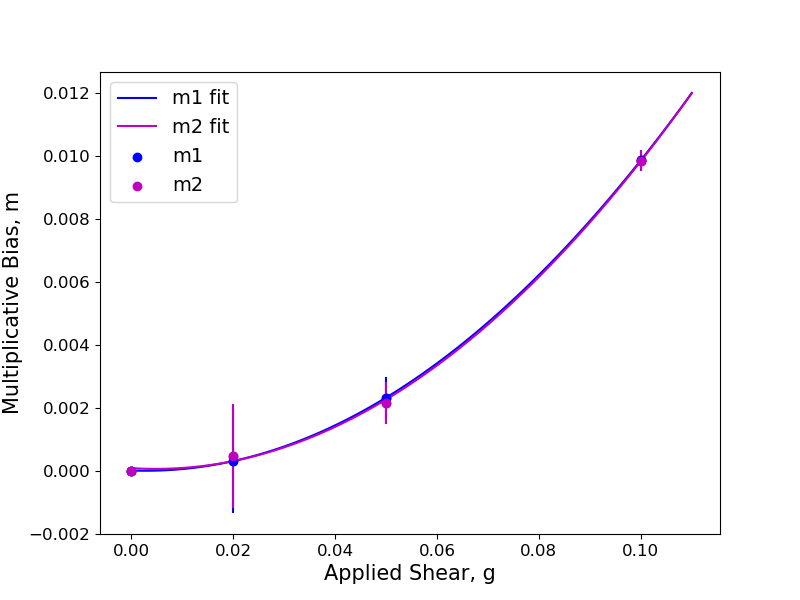
\includegraphics[width=\columnwidth]{metacal_bias_shear.png}
    \vspace*{-5mm}
    \caption{It shows the quadratic relationship between the input gravitational shear for the simple simulations and the multiplicative bias estimated from the recovered shape in the \textsc{metacalibration} catalogs. }
    \label{fig:metacal_shear_linear}
\end{figure}

\section{Results}
\label{sec:results}
In this section, we present the characteristics of the simulated data products. We divide our shape measurements into two categories; single-band and multiband. For single-band measurements, in each filter, we measure the shapes from the original single exposures by joint-fitting them. We set our base case to be this single-band joint-fit measurement. As the more developed case, we measure shapes with the single-band coadd in each filter by single-fitting it. For one multiband measurement, we match the objects, accumulate the single exposures from each filter catalog and measure the shapes with the joint-fit. The other multiband measurement joint-fit the three coadds from each filter together to recover the shape. 


From the COSMOS catalog, based on the \emph{Roman} Weak Lensing mission requirements, objects are pre-selected and simulated. In total, we simulate 907,170 galaxies on 18 SCAs across 198 pointings for F184, 227 pointings for H158, and 238 pointings for J129 bandpass. We do not make any selection cuts on the simulated catalogs based on measured properties. Even so, due to the misestimation of the PSF or low S/N, the Gaussian mixture fit with \textsc{ngmix} fails about 5\% of all simulated objects, and so the total number of the recovered objects for single-band measurements is, 861,960 for F184, 863,358 for H158, and 859,645 for J129. For the multiband (H158+J129+F184) coadd measurements, we measure objects that are covered by all of the filters and the total number of the recovered objects is 851,821.
Here are the measured properties of the objects in the \textsc{metacalibration} shape catalogs. 


% (galaxy and PSF properties; SNR, $e_{1,psf}$, $e_{2,psf}$, PSF FWHM) 
% havent decided on which plot to use. 
% \begin{figure}
% 	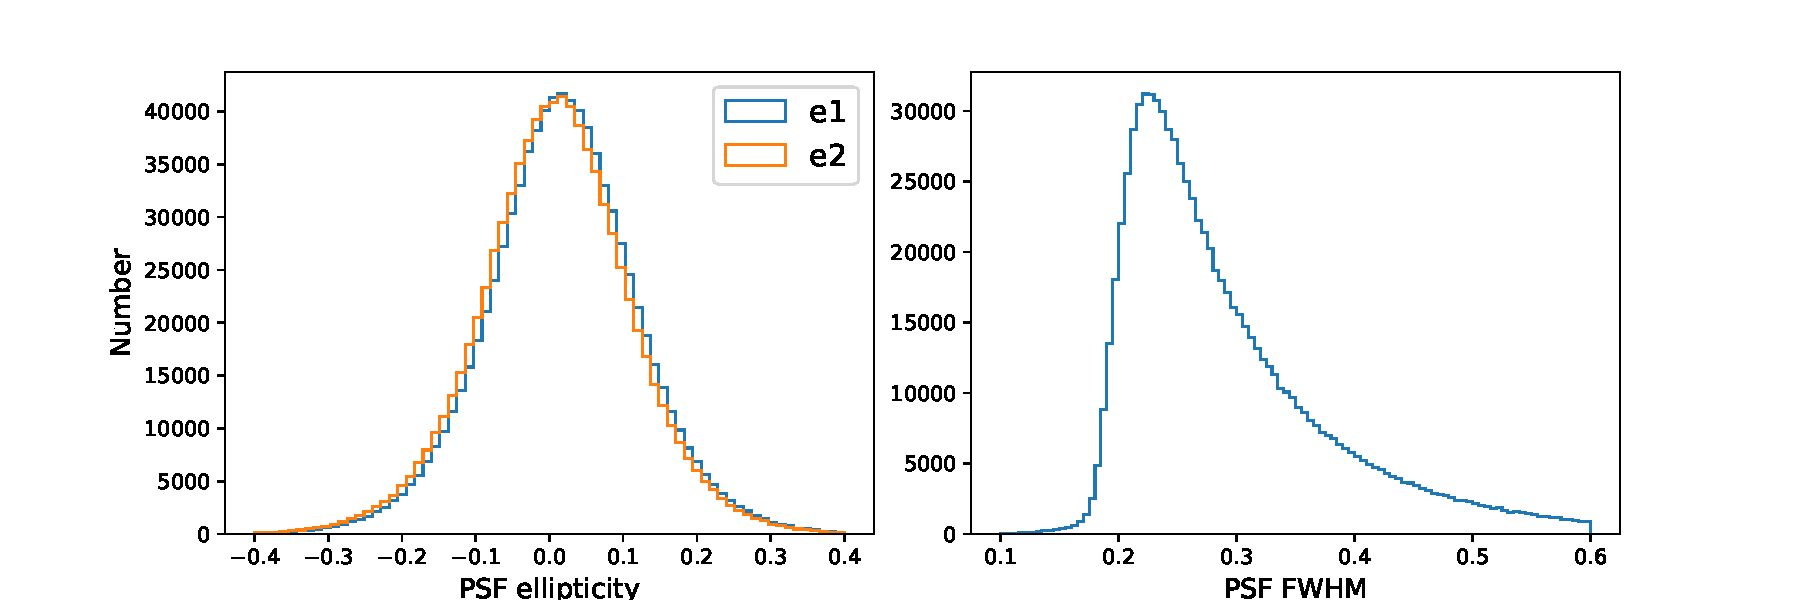
\includegraphics[width=\columnwidth]{figure5.pdf}
%     \caption{}
%     \label{fig:psf_properties}
% \end{figure}
% \begin{figure}
% 	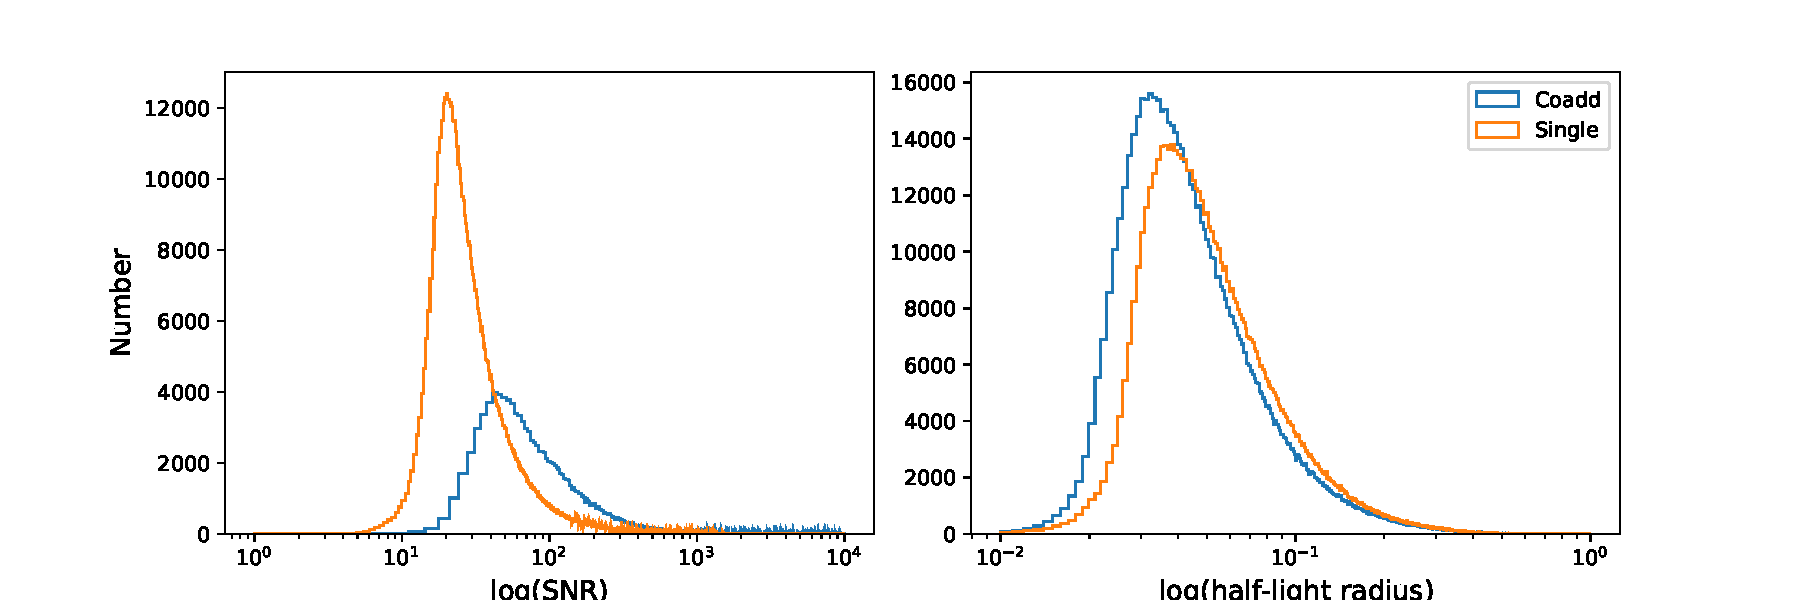
\includegraphics[width=\columnwidth]{figure6.pdf}
%     \caption{}
%     \label{fig:other_properties}
% \end{figure}


\subsection{Shape Calibration Bias}
\label{subsec:shapes}
We compute the estimated values of multiplicative and additive bias from the recovered shear with \textsc{metacalibration}. The results from the complete set of different runs are in Table \ref{tab:bias_summary} and the summary plot can be found in Figure \ref{fig:final_result}.  

For the single-band measurements, we can use the sampling factor defined in Equation \ref{eqn:sampling} to visualize the relationship between the sampling factor and the shear bias. The sampling factor is an indication of how undersampled the image in the filter is and it is respectively $Q_{J129}=1.01, Q_{H158}=1.23, Q_{F184}=1.44$. This was previously explored in \citealt{2021MNRAS.502.4048K}, where they found that the estimates shear bias has a large dependence on the sampling factor. We note that we have run \textsc{metacalibration} with \texttt{fitgauss} and \texttt{gauss} parameters for the new PSF model, and we found that it is preferrable to use \texttt{gauss} for our case. Hence, from here we present the result that is calibrated with \texttt{gauss} PSF model for \textsc{metacalibration}. The multiplicative bias of single-band single-epochs measurements for each filter is, 1.04$\pm$0.47 per cent for J129, -1.30$\pm$0.46 per cent for H158 and -0.40$\pm$0.53 per cent for F184. When the coadds of each filter are used, the bias becomes, -0.47$\pm$0.49 per cent for J129, -0.07$\pm$0.45 per cent for H158 and -0.06$\pm$0.61 per cent for F184. Coadd results are consistent with zero multiplicative bias within 1 sigma and the signals increase by xx per cent. Generally, coadding produces better sampled images as in Figure\ref{fig:single_to_coadd_rgb} and less multiplicative bias than single epochs measurements. We can conclude that in the \emph{Roman} simulation we have seen that the multiplicative bias has no strong dependence on the sampling factor.


Meanwhile the measured additive bias is the same level as the Y3 analysis in DES. The additive bias of the single-band single-epochs measurements for each filter is, (3.22$\pm$0.92)$10^{-4}$ for J129, (2.63$\pm$0.88)$10^{-4}$ for H158 and (3.25$\pm$1.11)$10^{-4}$ for F184. When the coadds of each filter are used, the bias becomes, (3.39$\pm$0.90)$10^{-4}$ for J129, (8.08$\pm$0.87)$10^{-4}$ for H158 and (9.36$\pm$1.10)$10^{-4}$ for F184. From the Table \ref{tab:bias_table}, it is worth noting that the coadd process clearly introduces non-trivial additive biases in one direction, but not the other. We believe this is due to the effect of an imperfect PSF model. We see this in the Figure xx where the recovered shear has a strong linear dependence on the PSF ellipticity measured by an adaptive moments method. The impact of the PSF leakage can be estimated by computing $\rho$-statistics (\citealt{2008A&A...484...67P, 2010MNRAS.404..350R, 2016MNRAS.460.2245J}). However, we do not explore the $\rho$-statistics for our PSF model since it is an approximation to accurately represent the features of the instrument, not computed from the real pupil plane images, and the coadding scheme for the 5-year mission has not been finalized yet. 


Next, we pressent the results with multiband measurements. We performed multiband measurements with 3 filters used in the previous measurements. One multiband measurement used all of the single epoch images from all the filters and joint-fit the shape of the galaxy. The multiplicative and additive bias is, respectively, $m=(-0.70\pm0.39)$ per cent and $c=(2.96\pm0.85)10^{-4}$. The other measurement performed the joint-fit on the three coadded image for each filter. The multiplicative and additive bias is, respectively, $m=(-0.59\pm0.46)$ per cent and $c=(7.78\pm0.94)10^{-4}$. The multiplicative bias is reduced but the additive bias increased due to the imperfect PSF modeling in one of the spin-2 axes. 



\begin{figure*}
	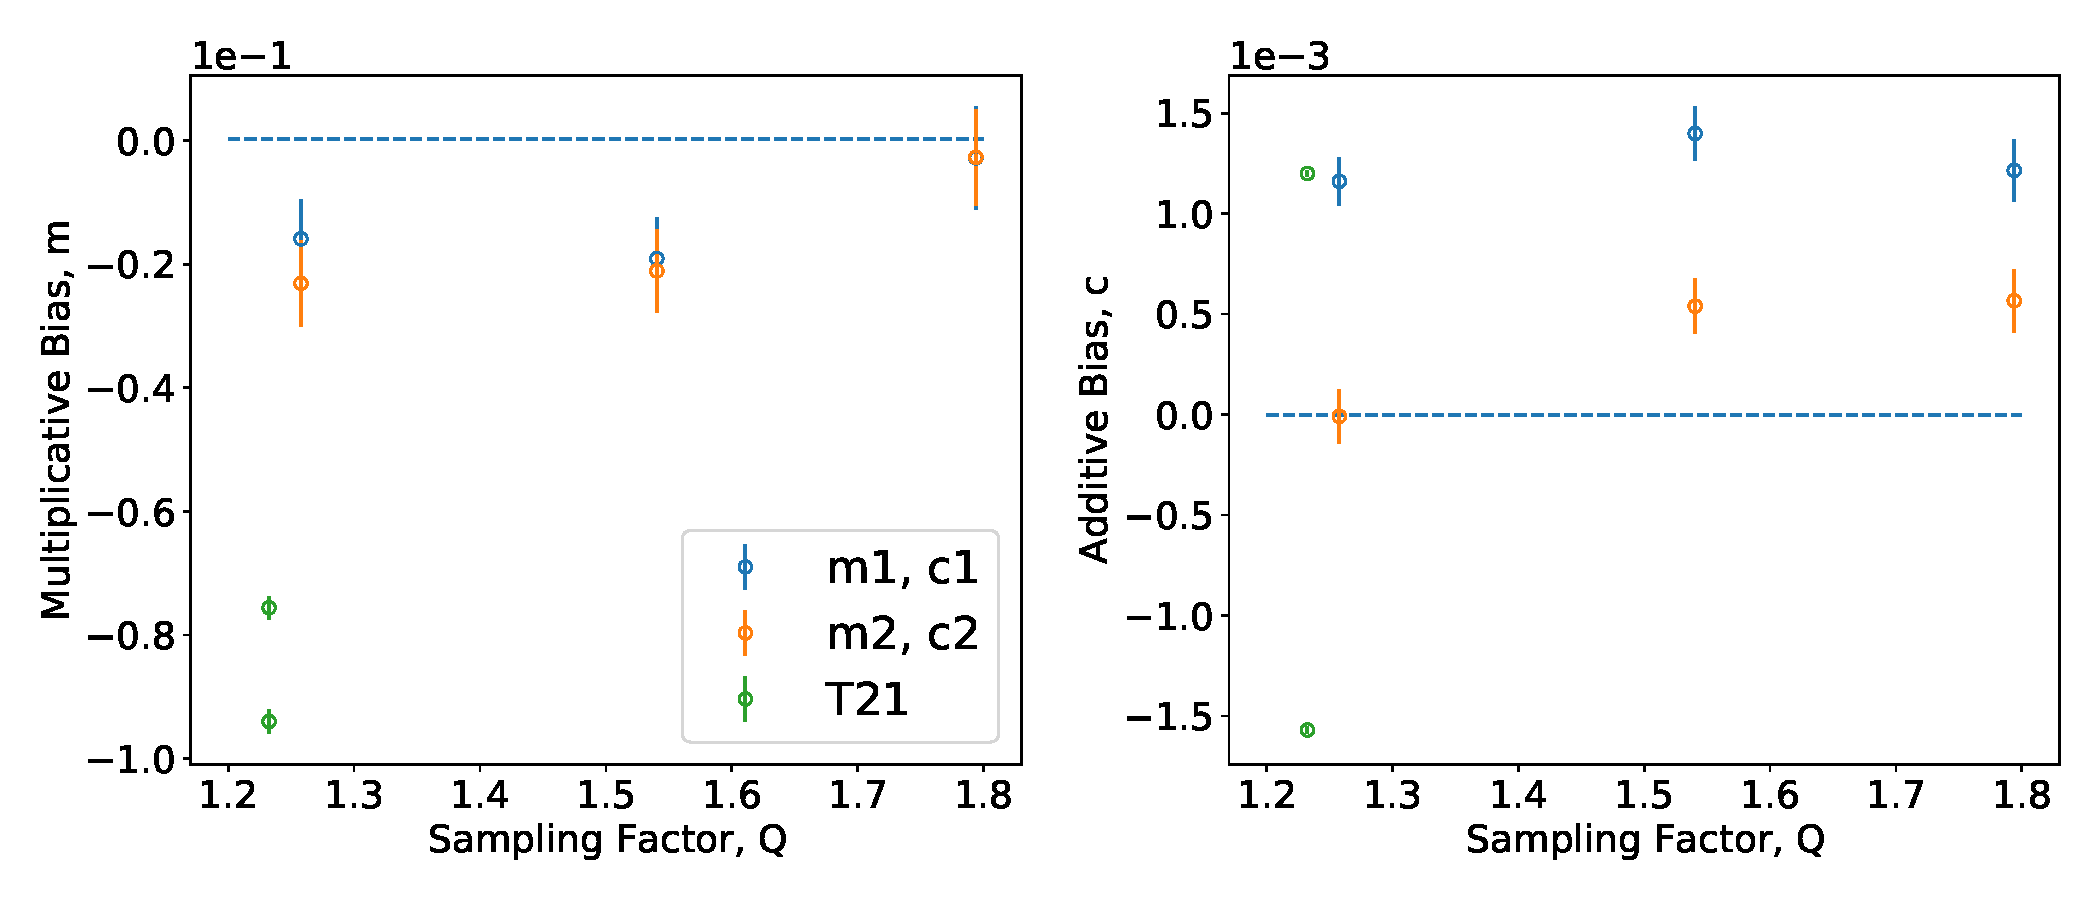
\includegraphics[width=\textwidth]{final_result.pdf}
    \caption{The multiplicative ($m$) and additive ($c$) bias of several simulation runs. The left panel shows $m$ and $c$ against the sampling factor for each filter. The right panel shows the same for multiband fit result. The number in the parenthesis gives how many filters are used. (3) means J129, H158 and F184 are used, whereas (2) means only J129 and H158 are used. Include the definition of sampling factor. }
    \label{fig:final_result}
\end{figure*}


\begin{table*}
	\centering
	\label{tab:bias_summary}
	\begin{tabular}[width=0.9*\textwidth]{ c|c|c|c|c|c } 
		\hline
		Bands & simulation variants & $m_{1}\times10^{-2}$ & $m_{2}\times10^{-2}$ & $c_{1}\times10^{-4}$ & $c_{2}\times10^{-4}$\\
		\hline
		\multirow{single-band} & single-epochs (J129) & 1.80$\pm$0.67 & 0.28$\pm$0.69 & 6.48$\pm$1.31 & -0.04$\pm$1.51\\
		& single-epochs (F184) & -0.62$\pm$0.81 & -0.17$\pm$0.79 & 3.92$\pm$1.52 & 2.58$\pm$1.57\\
		& single-epochs (H158; w/o noise fix) & -1.09$\pm$0.63 & -1.50$\pm$0.68 & 3.90$\pm$1.21 & 1.37$\pm$1.28\\
		& single-epochs (H158; w/ noise fix) & -1.18$\pm$0.63 & -1.43$\pm$0.67 & 2.14$\pm$1.35 & 1.83$\pm$1.19\\
		& single-band coadd with oversampling (H158; w/o noise fix) & -0.03$\pm$0.59 & -0.11$\pm$0.67 & 14.10$\pm$1.24 & 2.05$\pm$1.42\\
		& single-band coadd with oversampling (H158; w/ noise fix) & -1.51$\pm$0.68 & -1.41$\pm$0.66 & 14.79$\pm$1.32 & 4.45$\pm$1.42\\
		& single-band coadd with oversampling (H158; w/ noise fix, original pixel scale) & -5.89$\pm$0.72 & -5.53$\pm$0.64 & 2.54$\pm$1.25 & 3.09$\pm$1.21\\
		& single-band coadd with oversampling (H158; w/ noise fix, original pixel scale, diff draw) & -5.49$\pm$0.70 & -5.99$\pm$0.62 & 3.19$\pm$1.20 & 411$\pm$1.33\\
		& single-band coadd with oversampling (J129) & -0.49$\pm$0.65 & -0.45$\pm$0.62 & 10.50$\pm$1.33 & -3.72$\pm$1.42\\
		& single-band coadd with oversampling (F184) & 0.47$\pm$0.80 & -0.59$\pm$0.81 & 12.40$\pm$1.67 & 6.32$\pm$1.82\\
		
		\multirow{multiband} & multiband single-epochs (gauss) (H158+J129+F184) & -0.66$\pm$0.58 & -0.74$\pm$0.59 & 4.32$\pm$1.17 & 1.60$\pm$1.16 \\
		& multiband coadd (gauss; H158+J129+F184; all noise fixed; use noise flag turned off) & -2.14$\pm$0.58 & -2.51$\pm$0.58 & 14.17$\pm$1.21 & 4.55$\pm$1.21\\
		& multiband coadd (gauss; H158+J129+F184; only F184 noise fixed; use noise flag turned off) & -0.61$\pm$0.66 & -0.57$\pm$0.69 & 14.03$\pm$1.25 & 1.54$\pm$1.22\\
		& multiband coadd (gauss; H158+J129; no noise fix) & -0.39$\pm$0.59 & -0.32$\pm$0.68 & 13.72$\pm$1.24 & 1.85$\pm$1.29\\
% 		& (v2) multiband coadd (gauss; H158+J129) & -0.36$\pm$0.45 & -0.35$\pm$0.43 & 11.45$\pm$0.93 & 1.83$\pm$0.98\\
		
		\hline
	\end{tabular}
	\caption{Shear calibration bias for different simulation runs.}
	\label{tab:result}
\end{table*}


\section{Discussion}
\label{sec:discussion}

So far we have seen how \textsc{metacalibration} handles the relatively undersampled \emph{Roman} images without the effect of blending. The proportion of blended galaxies in the COSMOS catalog is xx per cent and it has been found that the galaxy blending at different redshifts could introduce a significant shear-dependent detection bias when calibrated with \textsc{metacalibration} (\citealt{2020ApJ...902..138S}). In the future study, we should investigate the impact of blending in the image simulations to verify if \textsc{metacalibration} is practical in the real survey. 


In the next generation of the simulations, we would like to add the following updates or upgrade these parts of the simulation. 
\begin{itemize}
    \item Expand the simulated area by at least 8 times.
    \item Incorporate the detector effects observed in the real flight candidate detectors.
    \item Enable the detector effects to be on and off to measure their effects on the final cosmology result.
    \item Implement the object detection scheme.
    \item Implement a new coadding methodology which coadds the whole scene instead of individual stamp cutouts (e.g., \texttt{pizza-cutter}\footnote{\url{https://github.com/beckermr/pizza-cutter}})
    \item Implement selection cuts (e.g., S/N) in the shape catalog.
\end{itemize}
With these potential changes, we would like to produce a reference image and shape catalog that can be widely used by other communities. 


\section{Conclusions}
\label{sec:conclusion}
We explored the performance of \textsc{metacalibration} methodology with \textsc{psc} coadding scheme to reduce the shear calibration bias in the image simulation framework of the \emph{Roman} Space Telescope. Accurately characterizing how much shear bias exists in this framework is required to successfully complete the weak lensing program of the High-Latitude Survey of the \emph{Roman}. \par

By coadding the single-epoch images and oversampling the PSF for a better shape fit, we find that shear estimates with \textsc{metacalibration} are slightly biased within 1 sigma but within the mission requirement. We conclude that to further constrain the shear calibration bias in the simulation and determine if the \emph{Roman} mission will be able to use the current Stage-III imaging survey schemes, we need more simulation volume well beyond the 2.5 deg$^{2}$ area of the simulated sky. 



\section*{Acknowledgements}

We thank Matthew Becker, Erin Sheldon, and Arun Kannawadi for many useful discussions. This work was supported by xx funding agencies.

%%%%%%%%%%%%%%%%%%%%%%%%%%%%%%%%%%%%%%%%%%%%%%%%%%
% \section*{Data Availability}

 
% The inclusion of a Data Availability Statement is a requirement for articles published in MNRAS. Data Availability Statements provide a standardised format for readers to understand the availability of data underlying the research results described in the article. The statement may refer to original data generated in the course of the study or to third-party data analysed in the article. The statement should describe and provide means of access, where possible, by linking to the data or providing the required accession numbers for the relevant databases or DOIs.




%%%%%%%%%%%%%%%%%%%% REFERENCES %%%%%%%%%%%%%%%%%%

% The best way to enter references is to use BibTeX:

\bibliographystyle{mnras}
\bibliography{example} % if your bibtex file is called example.bib


% Alternatively you could enter them by hand, like this:
% This method is tedious and prone to error if you have lots of references
%\begin{thebibliography}{99}
%\bibitem[\protect\citeauthoryear{Author}{2012}]{Author2012}
%Author A.~N., 2013, Journal of Improbable Astronomy, 1, 1
%\bibitem[\protect\citeauthoryear{Others}{2013}]{Others2013}
%Others S., 2012, Journal of Interesting Stuff, 17, 198
%\end{thebibliography}

%%%%%%%%%%%%%%%%%%%%%%%%%%%%%%%%%%%%%%%%%%%%%%%%%%

%%%%%%%%%%%%%%%%% APPENDICES %%%%%%%%%%%%%%%%%%%%%

\appendix

% \section{Coadding of F184 single epochs}
% \label{app:coadd_F}
% If you want to present additional material which would interrupt the flow of the main paper,
% it can be placed in an Appendix which appears after the list of references.

% \begin{table*}
% 	\centering
% 	\label{tab:bias_F}
% 	\begin{tabular}[width=0.9*\textwidth]{ c|c|c|c|c } 
% 		\hline
% 		simulation variants & $m_{1}\times10^{-2}$ & $m_{2}\times10^{-2}$ & $c_{1}\times10^{-4}$ & $c_{2}\times10^{-4}$\\
% 		\hline
% 		single-epochs (F184) & -0.62+-0.81 & -0.17+-0.79 & 3.92+-1.52 & 2.58+-1.57\\
% 		single-band coadd (F184) & 4.62$\pm$0.80 & 5.09$\pm$0.88 & -2.16$\pm$1.61 & -4.19$\pm$1.69\\
% 		single-band coadd with oversampling (F184) & 0.47$\pm$0.80 & -0.59$\pm$0.81 & 12.40$\pm$1.67 & 6.32$\pm$1.82\\
% 		multiband coadd with oversampling (F184+H158+J129) & 2.29$\pm$0.73 & 2.74$\pm$0.73 & 18.24$\pm$1.52 & 0.72$\pm$1.52\\
% 		\hline
% 	\end{tabular}
% 	\caption{Shear calibration bias for different simulation runs.}
% \end{table*}

% fitgauss or gauss appendix
% \begin{table*}
% 	\centering
% 	\label{tab:bias_table}
% 	\begin{tabular}[width=0.9*\textwidth]{ c|c|c|c|c|c } 
% 		\hline
% 		Bands & simulation variants & $m_{1}\times10^{-2}$ & $m_{2}\times10^{-2}$ & $c_{1}\times10^{-4}$ & $c_{2}\times10^{-4}$\\
% 		\hline
% 		\multirow{single-band} & single-epochs (J129) & 1.80$\pm$0.67 & 0.28$\pm$0.69 & 6.48$\pm$1.31 & -0.04$\pm$1.51\\
% 		& single-epochs (H158) & -1.09$\pm$0.63 & -1.50$\pm$0.68 & 3.90$\pm$1.21 & 1.37$\pm$1.28\\
% 		& single-epochs (F184) & -0.62$\pm$0.81 & -0.17$\pm$0.79 & 3.92$\pm$1.52 & 2.58$\pm$1.57\\
% 		& single-band coadd with oversampling (J129) & -0.49$\pm$0.65 & -0.45$\pm$0.62 & 10.50$\pm$1.33 & -3.72$\pm$1.42\\
% 		& single-band coadd with oversampling (H158) & -0.03$\pm$0.59 & -0.11$\pm$0.67 & 14.10$\pm$1.24 & 2.05$\pm$1.42\\
% 		& single-band coadd with oversampling (F184) & 0.47$\pm$0.80 & -0.59$\pm$0.81 & 12.40$\pm$1.67 & 6.32$\pm$1.82\\
		
% 		\multirow{multiband} & multiband single-epochs (fitgauss) (H158+J129+F184) & 1.78$\pm$0.62 & 0.07$\pm$0.63 & 8.80$\pm$1.22 & 1.57$\pm$1.27 \\
% 		& multiband single-epochs (gauss) (H158+J129+F184) & -0.66$\pm$0.58 & -0.74$\pm$0.59 & 4.32$\pm$1.17 & 1.60$\pm$1.16 \\
% 		& multiband coadd with oversampling (fitgauss; H158+J129) & -1.02$\pm$0.63 & 0.02$\pm$0.70 & 18.51$\pm$1.36 & 0.70$\pm$1.33\\
% 		& multiband coadd with oversampling (gauss; H158+J129) & -0.39$\pm$0.59 & -0.32$\pm$0.68 & 13.72$\pm$1.24 & 1.85$\pm$1.29\\
% 		& (v2) multiband coadd with oversampling (fitgauss; H158+J129) & -0.73$\pm$0.45 & -0.08$\pm$0.48 & 15.80$\pm$0.88 & 0.53$\pm$0.96\\
% 		& (v2) multiband coadd with oversampling (gauss; H158+J129) & -0.36$\pm$0.45 & -0.35$\pm$0.43 & 11.45$\pm$0.93 & 1.83$\pm$0.98\\
		
% 		\hline
% 	\end{tabular}
% 	\caption{Shear calibration bias for different simulation runs.}
% 	\label{tab:result}
% \end{table*}

%%%%%%%%%%%%%%%%%%%%%%%%%%%%%%%%%%%%%%%%%%%%%%%%%%


% Don't change these lines
\bsp	% typesetting comment
\label{lastpage}
\end{document}

% End of mnras_template.tex
